\subsection{Fluid and Particle Representations} \label{sec:fluidpart}
\begin{figure}
\centerline{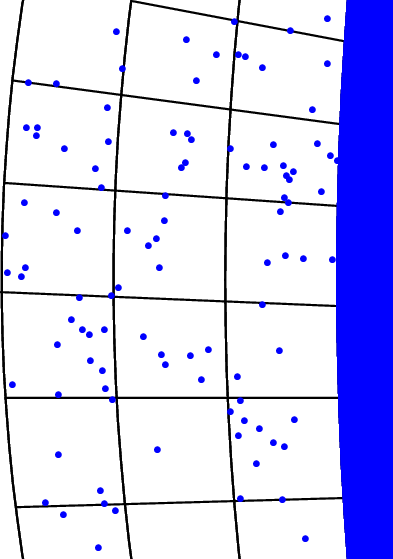
\includegraphics[width=6cm]{../pics/blpclonm}}
\caption{Wall at right, schematic finite element~(fe) mesh shown as distorted grid.
Plasma with fluid properties discretised using fe, interacts with neutral particle species
shown as dots.\label{fig:pcleover}}
\end{figure}
\begin{figure}
\centerline{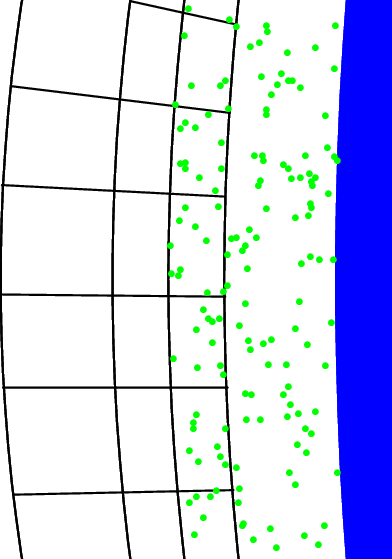
\includegraphics[width=6cm]{../pics/grpclovm}}
\caption{Handling a plasma sheath adjacent to wall at right.
Plasma has fluid properties discretised using fe indicated using warped grid,
but in sheath is better represented as particles indicated by dots.\label{fig:pcleadj}}
\end{figure}

As described in \Sec{intro}, there are two major distinct coupling cases. \Fig{pcleover}
shows is a common case where
plasma is represented on a mesh as a fluid whereas the neutrals are represented as
particles. \Fig{pcleadj} sketches a case where collisionality changes say because of sheath
formation, so there is a need to change representation depending on position. Note that
the mesh and particles are nonetheless shown as overlapping. This is believed to be good for numerical
robustness in enabling a smoother transition between two very different velocity-space distributions.
Both cases are found in engineering fluid dynamics, the first for example when treating combustion
products, the second occurs in stratospheric re-entry of space vehicles, although typically 
the fluid region is adjacent to the solid surface and long mean-free-paths are found at
distance. The overlap region in \Fig{pcleadj}
has attracted attention in the plasma context, leading to the particle-fluid model of
R\"{o}nnmark and Hamrin and the fluid-kinetic PIC model both as described in ref~\cite{Ma14Flui}.
The work of Taitano et al~\cite{Ta13Deve} appears to be more sophisticated, and 
subsequently has been generalised as the multiscale high-order/low-order (HOLO) algorithm
which could also address issues around Model Order Reduction~\cite{Ch17Mult}.

\subsection{Advanced Sampling Techniques} \label{sec:sampling}
The drawback of the particle approach~PIC is potentially the low arithmetic intensity 
relative to accuracy because of the well-known scaling of error$\propto 1/\sqrt{N_p}$ for
Monte-Carlo-type methods using $N_p$ particles, which
may make PIC very inefficient at the Exascale.
The control-variates idea of using particles to simulate only
deviations from Maxwellian is already well-developed as the so-called $\delta f$ method,
see the review~\cite{Wa95a}. Present gyrokinetic codes are treating $N_p=10^{11}$ particles
in this way, although these calculations appear to be encountering difficulties.

\begin{figure}
\centerline{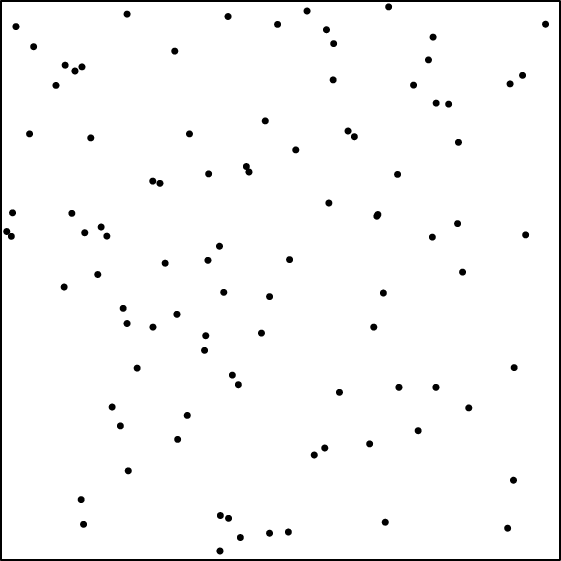
\includegraphics[width=8cm]{../png/ranlux1}}
\caption{Monte-Carlo sampling of points in a square\label{fig:ranlux1}}
\end{figure}
\begin{figure}
\centerline{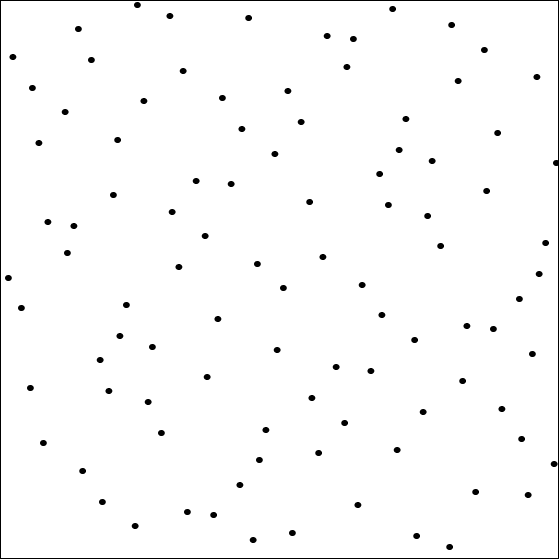
\includegraphics[width=8cm]{../png/halton1}}
\caption{Quasi-Monte-Carlo sampling of points in a square\label{fig:halton1}}
\end{figure}

Of course,
it will generally be good to reduce the number of particles required for a given error.
As illustrated by \Fig{ranlux1}, the purely random points from Monte-Carlo sampling
tend to cluster. If it is known that lengthscales below a certain critical value are
unimportant, then Quasi-Monte-Carlo sampling as indicated by \Fig{halton1} may do better, and here
errors scale closer to $1/N_p$ than $\propto 1/\sqrt{N_p}$. 
These more sophisticated sampling techniques are relatively immature in application to neutrals,
never mind plasma, but since sampling noise is often the main limiting factor, this simple
argument shows that they can be transformative and so cannot be ignored. Ameres~\cite{ameres}
has begun to examine this point both analytically and numerically, as earlier, assuming
periodicity in physical space.
%(The mention of sampling brings in uncertainty quantification, where careful sampling is
%an important tool, but there will be a separate task on UQ in which to report work
%on say MLMC and MIMC.)

There are also the hierarchical approaches MLMC~(Multi-Level Monte-Carlo) and MIMC (Multi-Index Monte-Carlo)
that offer the promise of efficiency gains~\cite{Ha18Mult}. PIC is formulated as a set of stochastic
differential equations known as a McKean-Vlasov process (meaning the coefficients of
the equation depend on expected values of its solution). However the gains appear to be much less
dramatic than for QMC~\cite{Ri15mult}.

\subsection{Implicit Particle Methods} \label{sec:implicit}
The HOLO schemes of \Sec{fluidpart} above, already require an implicit formulation.
In the context of purely PIC schemes, widely differing particle masses (masses of Hydrogen ions and electrons in a ratio
of nearly~$2000$) can also pose a challenge when it comes to coupling the species. 
Generally, given the possibility of widely
different timescales, an implicit approach is indicated which is more natural 
when there is coupling to a fe model that is also implicit.
However it could be important that the implicit particle method requires the solution of
matrices with dimensions that scale only with the mesh-size$\propto N^p_D$ where $p_D\leq 3$ is 
the spatial dimension, not with particle number~$N_p$. This has driven research by
the groups of Lapenta~\cite{Si18Comp} and Chacon~\cite{Ch11ener} into
approaches variously referred to as `particle enslavement' or `kinetic enslavement'.
It is significant that the efficiency of the approach depends on how the resulting matrix
equations are solved, with the choice of preconditioner's being important. 

\subsection{Timestep-Robust Particle Tracking} \label{sec:robupart}
For both ease of implementation and speed of execution, many researchers 
over many years have noted that it would be very desirable
to have a `stiff' particle-pusher, viz.\ an algorithm for integrating the equation of motion
of a charged particle in the electromagnetic field, that could produce accurate
trajectories regardless of timestep size. The canonical `Boris' pusher is only satisfactory
for timesteps significantly shorter than the gyro-period (the time taken for the particle to
oscillate about the local field direction). However often, for example leading to the large area 
of modelling work usually loosely referred to as
``gyrokinetics", details of the gyro-orbit are unimportant in the overall plasma simulation.

In the past two years alone, as a development of `Boris', Hairer~\cite{Ha19filt} has been
encouraged to look at use of the `filter' approach he has applied in other ODE integrators.
Chacon and Ricketson~\cite{Ri19ener} have examined the replacement of `Boris' by the implicit mid-point
rule, which is possible in the context of an implicit PIC code.
Burby~\cite{Bu20guid} has tackled the problem from the point-of-view of slow manifold theory.
%more tractable, it could be important to derive new formulae to advance the
%particles.
%  there are analytic formulae which average over gyration, and Hairer is exploring
%approximations that bridge the gap between average and exact helical trajectory.

\subsection{Exascale-related Issues} \label{sec:exasc}
At the SIAM PP20 meeting, it was pointed out that
for the Exascale, there are important issues which are common to
a broad range of particle problems. Reeve in Session MS64 gave a talk highlighting the Co-design center for Particle
Applications~(CoPA) that addresses issues common to many fields of particle simulation (such
as Molecular Dynamics and cosmology as well as PIC). It is worth noting that they see simulation
packages as being built in a series of layers, as illustrated by for example the CabanaMD package,
to maximise flexibility and the possibility for re-use. A significant point also is their
focus on data structures such as array-of-structs (AoS) and structs-of-arrays (SoA), as well
as array-of-structs-of-arrays (AoSoA). From the computational physicist's point-of-view this
focus on data structure elements such as arrays is unsatisfactory, in that the physics indicates that all the
information in a region of space represented by say a few fes should be co-located, which 
means for \nep \ , data from fields and particles' being re-ordered in quite a different manner.


For particle problems, presenters, notably Pope (for Habib in MS64), did mention the important of `tree'-based storage.
Guo in MS22 discussed the effects of using different storage strategies, but found  somewhat surprisingly 
changes in execution time of only approx.~$10$\,\%. However,
only of order a million particles were present. In the tokamak case, there is
also the issue that there may be many different species with different 
representations and spatial distributions.
